\documentclass{beamer}

\usepackage{amsmath, amssymb, hyperref, graphics}
\usepackage{mathpazo}

\newcommand{\C}{\mathbb{C}}
\newcommand{\Z}{\mathbb{Z}}


\title{Commutative Algebra MAS439 \\ Lecture 1}
\author{Paul Johnson \\ \href{mailto:paul.johnson@sheffield.ac.uk}{paul.johnson@sheffield.ac.uk} \\ Hicks J06b}
\date{September 28th}

\begin{document}

\begin{frame}
\titlepage
\end{frame}


\begin{frame}{Assessment is entirely via problem sets}

\begin{itemize}
\item Problems are due \emph{every} Wednesday at the \emph{beginning} of class
\item Each semester, the two lowest problem set scores can be dropped
\item You are encouraged, but not required, to write your solutions in \LaTeX
\item You are encouraged, but not required, to work together in groups of 2 or 3
\end{itemize}
\end{frame}


\begin{frame}{Wait, groupwork?! How does that work?}

\begin{itemize}
\item Each group member writes up and hands in their own solution
\item If you do work in groups, please write who you worked with on every assignment
\end{itemize}

\begin{block}{What is/isn't allowed:}
\begin{itemize}
\item You should \alert{NOT} be writing up identical solutions, or even writing up your solutions sitting together.  
\item Rather, in the group digest what the problem is actually asking, come up with an informal / pseudo-formal solution
\item \alert{LATER}, on your own, write up the full, rigorous solution
\end{itemize}
\end{block}

\end{frame}

\begin{frame}{Rigour and intuition, proof and understanding}

\begin{itemize}
\item Mathematics is all in our heads.  Giving formal definitions and rigorous proofs make sure we're not just making up nonsense
\item However, humans don't think very well in this rigorous structure.  We have our own intuitive pictures
\item Most of the work of doing mathematics is translating back and forth between rigorous and intuitive modes.
\end{itemize}


\begin{block}{The \emph{Oral tradition} in mathematics}
Mathematics is written down in full rigor, but informal discussion of ``how to think about this'' or  ``what's really going on'' aren't written down
\end{block}


\begin{itemize}
\item Terry Tao, \href{https://terrytao.wordpress.com/career-advice/there’s-more-to-mathematics-than-rigour-and-proofs/}{There's more to mathematics than rigour and proofs}
\item William Thurston, \href{https://arxiv.org/abs/math/9404236}{On proof and progress in mathematics}
\end{itemize}


\end{frame}


\begin{frame}{Lectures and Notes}

\begin{itemize}
\item  Primary text: Tom Bridgeland's notes (rigor)
\item I won't provide lecture notes (intuition)
\end{itemize}

\begin{block}{Weekly webpage}
\begin{itemize}
\item Terse description of what was covered in lecture
\item Slides
\item Problem set
\item Feedback on problem set?
\item Comment section
\end{itemize}
\end{block}




\end{frame}


\begin{frame}{The first 3-4 weeks should be somewhat review}

\begin{columns}
\column{.5\linewidth}
\begin{block}{MAS220 Syllabus from 2014}
 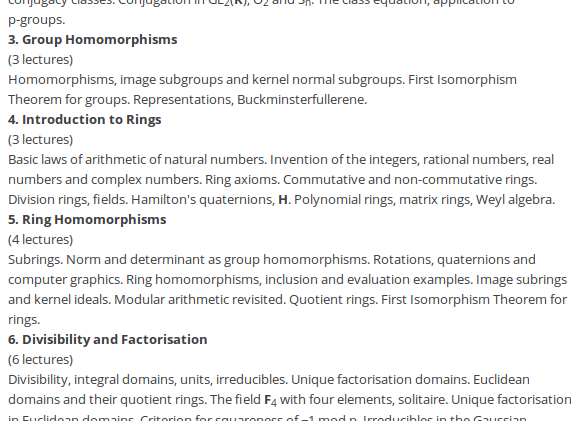
\includegraphics[width=.9\linewidth]{MAS220}
\end{block}
%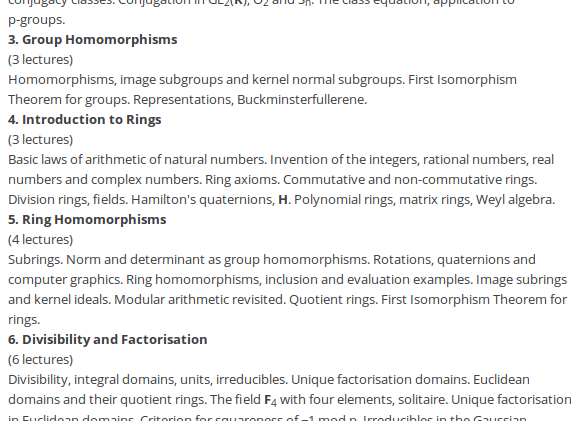
\includegraphics{MAS220}
\column{.5\linewidth}
\begin{block}{MAS439 Table of Contents}
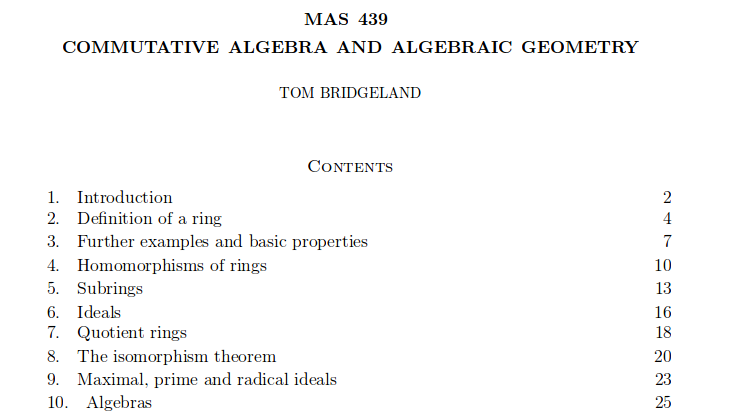
\includegraphics[width=.9\linewidth]{TOC}
\end{block}
\end{columns}
\begin{itemize}
\item You've forogtten a lot of this not having used it for two years
\item We do everything more in depth and sophisticated
\end{itemize}
\alert{I AM DEPENDING ON YOU TO LET ME KNOW IF I'M GOING TOO FAST} (or too slow)

\end{frame}



\begin{frame}{A quiz to see what you know}

Answer these questions to the best of your ability on the blank sheet of paper provided.

\begin{enumerate}
\item What's the formal definition of a ring homomorphism?  Give an example.
\item What's the formal definition of an ideal?  What's the \emph{point} of this definition?
\item Give at least 5 examples of rings.
\end{enumerate}

Up to you whether you put your name on them or not; I'm just using these as a quick gauge of our background.

\end{frame}

\begin{frame}{Definition of a ring}

A \emph{ring} is a set $R$ with two binary operations $+, \cdot$ on $R$ satisfying:

\begin{enumerate}
\item $\forall x, y,z\in R, (x+y)+z=x+(y+z)$
\item $\exists 0_R\in R$ such that $\forall x\in R,  0_R+x=x+0_R=x$
\item $\foral x\in R, \exists {-x}\in R$ such that $x+({-x})=({-x})+x=0_R$
\item $\forall x,y \in R, x+y=y+x$
\item $\forall x, y,z\in R, (x\cdot y)\cdot z=x\cdot (y\cdot z)$
\item $\exists 1_R\in R$ such that $\forall x\in R, 1_r\cdot x=x\cdot 1_R=x$
\item $\forall x, y,z\in R, x\cdot (y+z)=x\cdot y+x\cdot z$ and $(y+z)\cdot x=y\cdot x+ y\cdot z$
\end{enumerate}

\end{frame}

\begin{frame}{Definition of a ring, take two}
A \emph{ring} is a set $R$ with two binary operations $+,\cdot$ satisfying:

\begin{enumerate}
\item $(R,+)$ is an abelian group
\item $(R,\cdot)$ is a monad
\item Multiplication $(\cdot)$ distributes over addition $(+)$
\end{enumerate}

A \emph{monad} satisfies all the axioms of a group except perhaps the existence of inverses.
\end{frame}

\begin{frame}{Examples of rings}
\begin{enumerate}
\item The trivial ring has one element
\item The integers $\mathbb{Z}$
\item Any field $\mathbb{Q}, \mathbb{R}, \mathbb{C}, \mathbb{F}_2, \cdots$
\item ``clock arithmetic'' $\mathbb{Z}/12\mathbb{Z}$ and more generally $\mathbb{Z}/n\mathbb{Z}$
\item Polynomial rings $\mathbb{R}[x], \mathbb{\Z}[y,z]$
\item The set $M_n(\mathbb{R})$ of $n\times n$ matrices with real coefficients
\item The quaternions $\mathbb{H}$
\item The Gaussian integers $\mathbb{Z}[i]=\{z=a+bi\in \mathbb{C} | a,b\in \mathbb{Z}\}$
\item The set $\text{Fun}(\mathbb{R}, \mathbb{R})$ of all functions from $\mathbb{R}$ to itself, under pointwise addition and multiplication (e.g., $(f\cdot g)(x)=f(x)\cdot g(x)$)
\item The set $C(\mathbb{R})$ of all \emph{continuous} functions from $\mathbb{R}$ to itself
\end{itemize}
\end{frame}


\begin{frame}{Commutative algebra is the study of commutative rings}

\begin{definition}
A ring $R$ is \emph{commutative} if multiplication is commutative, i.e. $x\cdot y=y\cdot x$
\end{definition}

\begin{block}{Convention:}
Unless otherwise specified, all rings $R$ will be assumed to be commutative.
\end{block}


\end{frame}


\end{document}
